% ----------------------------------------------------------------
% achemso --- Support for submissions to American Chemical
%  Society journals
% Maintained by Joseph Wright
% E-mail: joseph.wright@morningstar2.co.uk
% Originally developed by Mats Dahlgren
%  (c) 1996-98 by Mats Dahlgren
%  (c) 2007-2008 Joseph Wright
% Released under the LaTeX Project Public license v1.3c or later
% See http://www.latex-project.org/lppl.txt
% 
% Part of this bundle is derived from cite.sty, to which the
% following license applies:
%   Copyright (C) 1989-2003 by Donald Arseneau
%   These macros may be freely transmitted, reproduced, or
%   modified provided that this notice is left intact.
% ----------------------------------------------------------------
% 
% The achemso bundle provides a LaTeX class file and BibTeX style
% file in accordance with the requirements of the American
% Chemical Society.  The files can be used for any documents, but
% have been carefully designed and tested to be suitable for
% submission to ACS journals.
% 
% The bundle also includes the natmove package.  This package is
% loaded by achemso, and provides automatic moving of superscript
% citations after punctuation.

\documentclass[
%journal=ancac3, % for ACS Nano
%journal=acbcct, % for ACS Chem. Biol.
journal=jpcbfk, % for undefined journal
manuscript=article]{achemso}

\usepackage[version=3]{mhchem} % Formula subscripts using \ce{}
\usepackage{graphicx}
\usepackage{caption}
\usepackage{subcaption}
\usepackage[labelfont={bf}]{caption}
\usepackage{minted}

\newcommand*{\mycommand}[1]{\texttt{\emph{#1}}}

\author{Trerayapiwat K.}
\email{ktreraya@bowdoin.edu}
\affiliation[Bowdoin College]
{Department of Chemistry, Bowdoin College, Brunswick, ME}
\author{Eustis S.}
\email{seustis@bowdoin.edu}
\affiliation[Bowdoin College]
{Department of Chemistry, Bowdoin College, Brunswick, ME}


\title[\texttt{achemso} demonstration]
{Benchmarking Ab Initio Computational Methods for the Quantitative Prediction of Sunlight-Driven Pollutant Degradation in Aquatic Environments}

\begin{document}


\begin{abstract}
Understanding of the changes in molecular electronic structure following the absorption of light is a fundamental challenge for the goal of predicting photochemical rates and mechanisms. Excitation energies and oscillator strengths were calculated using different theories and methods. A new approach was selected to model the photon absorption: Molecular Dynamics–Time Dependent Density Functional Theory (MD-TD-DFT). An aniline molecule equilibrates in the presence of a number of water molecules at room temperature using 6-311++G** basis set. Excitation energy and oscillator strength of aniline geometries in equilibrium are then calculated using TD-DFT with CAMB3LYP, or M06-2X functional. The computed physical properties from MD-TD-DFT then compared with data from experimental absorption spectra to evaluate the accuracy of the two methods. Absorption spectra’s underlying modified Gaussian functions were decomposed and integrated to calculate experimental oscillator strength at a certain excitation energy using an R code written by Peter Cohen.
\end{abstract}


\section{Introduction}

\subsection{Environmental Photochemistry And Micropollutants}

During the past century, more and more synthetic chemicals has been created for commercial pharmaceuticals and personal care products. Each year, about 300 million tons of organic chemicals are being added into water systems.\cite{Schwarzenbach2006} These chemicals has been detected in ng/L to μg/L in the aquatic systems worldwide.\cite{Monteiro2010} The scale of chemicals being introduced into the water reaffirms the need for close studies in order to understand the consequences of these compounds on the environmental system, and eventually to living beings. While major toxic chemicals, such as \ce{CCl4}, DDT etc., has been constantly regulated or banned by governments for its effects on agriculture and the environment, many more compounds have not received the attention they deserve. Even though some are approved as safe for daily usage in household products, their impacts after being disposed into water remain largely unknown due to exhaustive amount of effort to study all the compounds. These low-concentration chemicals are collectively called mictopollutants. However, small concentration, large number of different types, difficulty separating or concentrating for analysis contribute retard the effort to understand their effects on in water systems. Nevertheless, detectable decrease in concentration of micropollutants in downstream of rivers close discharge areas compared to upstream has been identified to be mainly from photolysis under UV-C.\cite{Conley2008,Daneshvar2010,Bonvin2011,Carlson2015} Some photodegrade into more toxic species. Triclosan, which been used as an anti-bacterial agent in household soap and health care products decomposes under sunlight to Dioxins and PCBs, well-known carcinogens.\cite{Bedoux2012} Previously, computational studies of Triclosan in the excited states were carried out by Soren N. Eustis.\cite{Kliegman2013} Within Eustis lab, Nathan Ricke worked on applying computational model to estimate quantum yields of photoexcited small organic molecules.\cite{Ricke2014} 

\subsection{Computational approach, Photoexcitation, and UV-VIS Spectrum}
In the recent years, computer has become more and more accessible to researchers.\cite{Dykstra2011} The power of High Performance Computer (HPC) expands the universe of rigorous computational calculations to analytically unsolvable quantum problems. Moving away from semi-empirical models, computational chemists can now implement Ab Initio methods using fundamental equations, which decades before, was prohibited by the high computational time and resources. In studying photodegradation in micropollutants, computational approach allows for a priori prediction of photoproducts and their impact on the environment instead of posteriori study of damage done, not to mention the complexity and limitations of experimental designs in order to study individual species of micropollutants. In natural water, many species of micropollutants interfere with each other putting limits on how much experimental approach can be used to study the natural system. 

\begin{figure}[htb]
	\centering		
	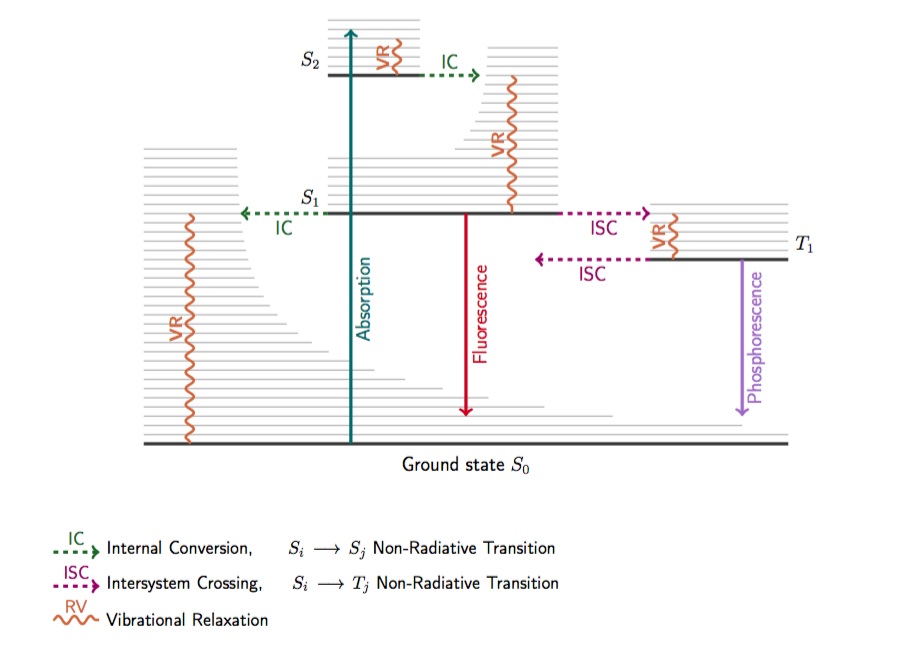
\includegraphics[width=1\textwidth]{jablonski.png}
	\caption{Jablonski diagram. A possible pathway of photoexcitation starts at ground state to singlet excited state, then triplet excited states.}
	\label{fig:jablonski}
\end{figure}
\begin{figure}[htb]
	\centering		
	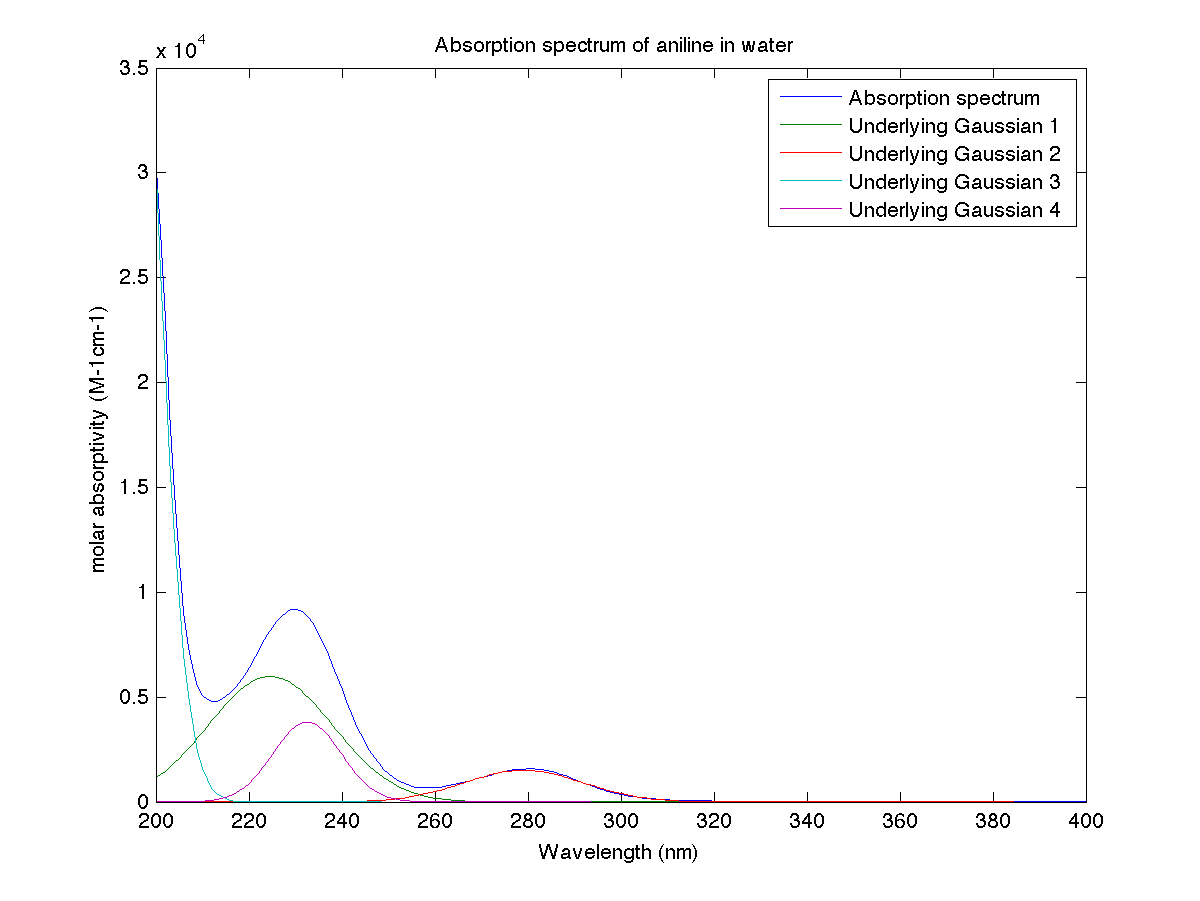
\includegraphics[width=1\textwidth]{UVFromFityk.png}
	\caption{Absorption spectrum of aniline in water with underlying Gaussian printed out. Program Fityk is used to fit these four Gaussian manually.}
	\label{fig:UVFromFityk}
\end{figure}
A molecule in its ground state can absorb a photon, transform to its first singlet excited state (S1), then its first triplet excited state (T1) as illutrated in figure \ref{fig:jablonski}. Triclosan at triplet states goes through photodegradation and decompose. Understanding transition from singlet to triplet state was studied previously in Eustis lab.\cite{Ricke2014} While reactions in excited state are important to understanding photochemical reaction, excitation from ground states by photons to exited states is equally important to understand complete reaction mechanism. Most familiarly, studying absorption of photons in chemical compounds are done through UV-VIS absorption spectra. A molar absorptivity vs wavenumber plot reveals excitation energies of electronic transitions in a particular species of chemical compound. In vapor, simulation of UV-VIS spectrum can be done more easily due to lack of solvent broadening.\cite{Hirayama2010} However, in linking UV-VIS spectrum with theory, a more fundamental value called oscillator strength should be used. Oscillator strength tells the degree of allowness of transition between two electronic states. Mathamatically, oscilator strength can be calculated from integrating molar absorptivity over a range of wavenumber within an electronic transition - see equation \ref{eq:oscillatorStrength}.
\begin{equation}
\label{eq:oscillatorStrength}
f = 4.39\times 10^{-9}\int_{\widetilde{\nu}_{a}}^{\widetilde{\nu}_{b}}\varepsilon(\widetilde{\nu}) d\widetilde{\nu}
\end{equation}
After calculation of excited state energies and the oscillator strength, computational results will be compared with experimental UV-VIS spectrum to evaluate accuracy of the models used. One another complication of the problem is the solvent broadening of absorbance peaks. As peaks are broadened, each individual peak combines together into a continuous experimental spectrum as in figure \ref{fig:UVFromFityk}. Integration cannot be done without deconvoluting the underlying Gaussians. Currently, matlab code utilizing Bayesian probability as a statistical technique to properly find the Gaussian plots are developed by professor Soren Eustis from previous work in R with Peter Cohen '18.

 There are currently no studies on quantitative calculation of excited state energies of organic molecule in water. This allows room for a systematic approach to develop an appropriate computational model that would allow for further understanding of aquatic pollutants.

\subsection{Solvent Models}

Despite recent advent of growth in computer speed and burgeoning interest in incorporating computational models to further understand the nature world, large systems such as solvation models remains a big challenge.\cite{Lin2007} In modeling effects of solvent molecules on solute, implicit solvation models were previously implemented because it allows for acceptable results calculation while maintaining good speed (low computational cost). Most famous of all implicit models is Potential Continuum Model (PCM).\cite{Cossi2000} Instead of explicitly handling each solvent molecule quantum mechanically, PCM expresses their bulk effects on solute molecule in means of dielectric continuum field surrounding molecule of interest. Its downfall is that, however, its accuracy falls short of static and dynamic contribution of excited states properties.\cite{Barone2007} Furthermore, implicit solvent model also neglects hydrogen-bonding as it assumes implicit implementation in dispersion forces and electrostatics.\cite{Li1999} Especially in calculating excited state energies, an accurate solvent model should be used.\cite{Tomasi2005} In explicit solvent model, one recent notable method – Effective Fragment Potentials (EFP) can be used to model explicit solvents with non-bonded van der Waals interactions, hydrogen bonding using Coulomb interactions, polarization, and exchange repulsion without high computational expense of explicit models.\cite{Day1996,Yoo2008} 

\subsection{Computational Models: Theories, Basis Sets, and Functionals}

Among all current theories, Time-Dependent Density Functional Theory (TD-DFT) is the most promising with its high accuracy when used with appropriate functionals and low computational cost\cite{Magyar2007}. Implementing EFP solvent model, TD-DFT can be used to accurately calculate excited state energy of acetone in water.\cite{Yoo2008} Typically in Implicit solvent model, geometry optimization of solute molecule is carried out with PCM, followed by calculation of excited state energies, also with PCM. This static ground state molecule however does not accurately represent solute in water.\cite{Defusco2011} Instead, Molecular Dynamics (MD) of solute and solvent fragments can be used to obtain a range of equilibrated structures for excited state energies calculation. Mark Gordon averaged the calculated energies of each excited state to arrive at a final excited states energy.\cite{Defusco2011}

According to previous basis set studies, wile having roughly the same computational cost, an average-sized basis set 6-311++G(2d,p) performs better than aug-cc-pVDZ (ACCD).\cite{Wiberg2004,Barnes2014} For example, transition energies calculated of CN molecule as calculated by ACCD deviates 1117-1669 cm\textsuperscript{-1} from experimental value while those by 6-311++G(2d,p) only deviate 220-470 cm\textsuperscript{-1}. In previous study, CAMB3LYP, M06-2X are reported to be one of the most reliable functionals in calculating vertical excitation energy (average root mean square deviation of 2272 cm\textsuperscript{-1}  and 2187 cm\textsuperscript{-1}  respectively compared to 3114 cm\textsuperscript{-1} for M06 and 18196 cm\textsuperscript{-1} for CIS).\cite{Barnes2014} 

\subsection{fd}

\section{Method}

\subsection{Overview}
Approach to develop a model for 
\begin{figure}[!htb]
	\centering		
	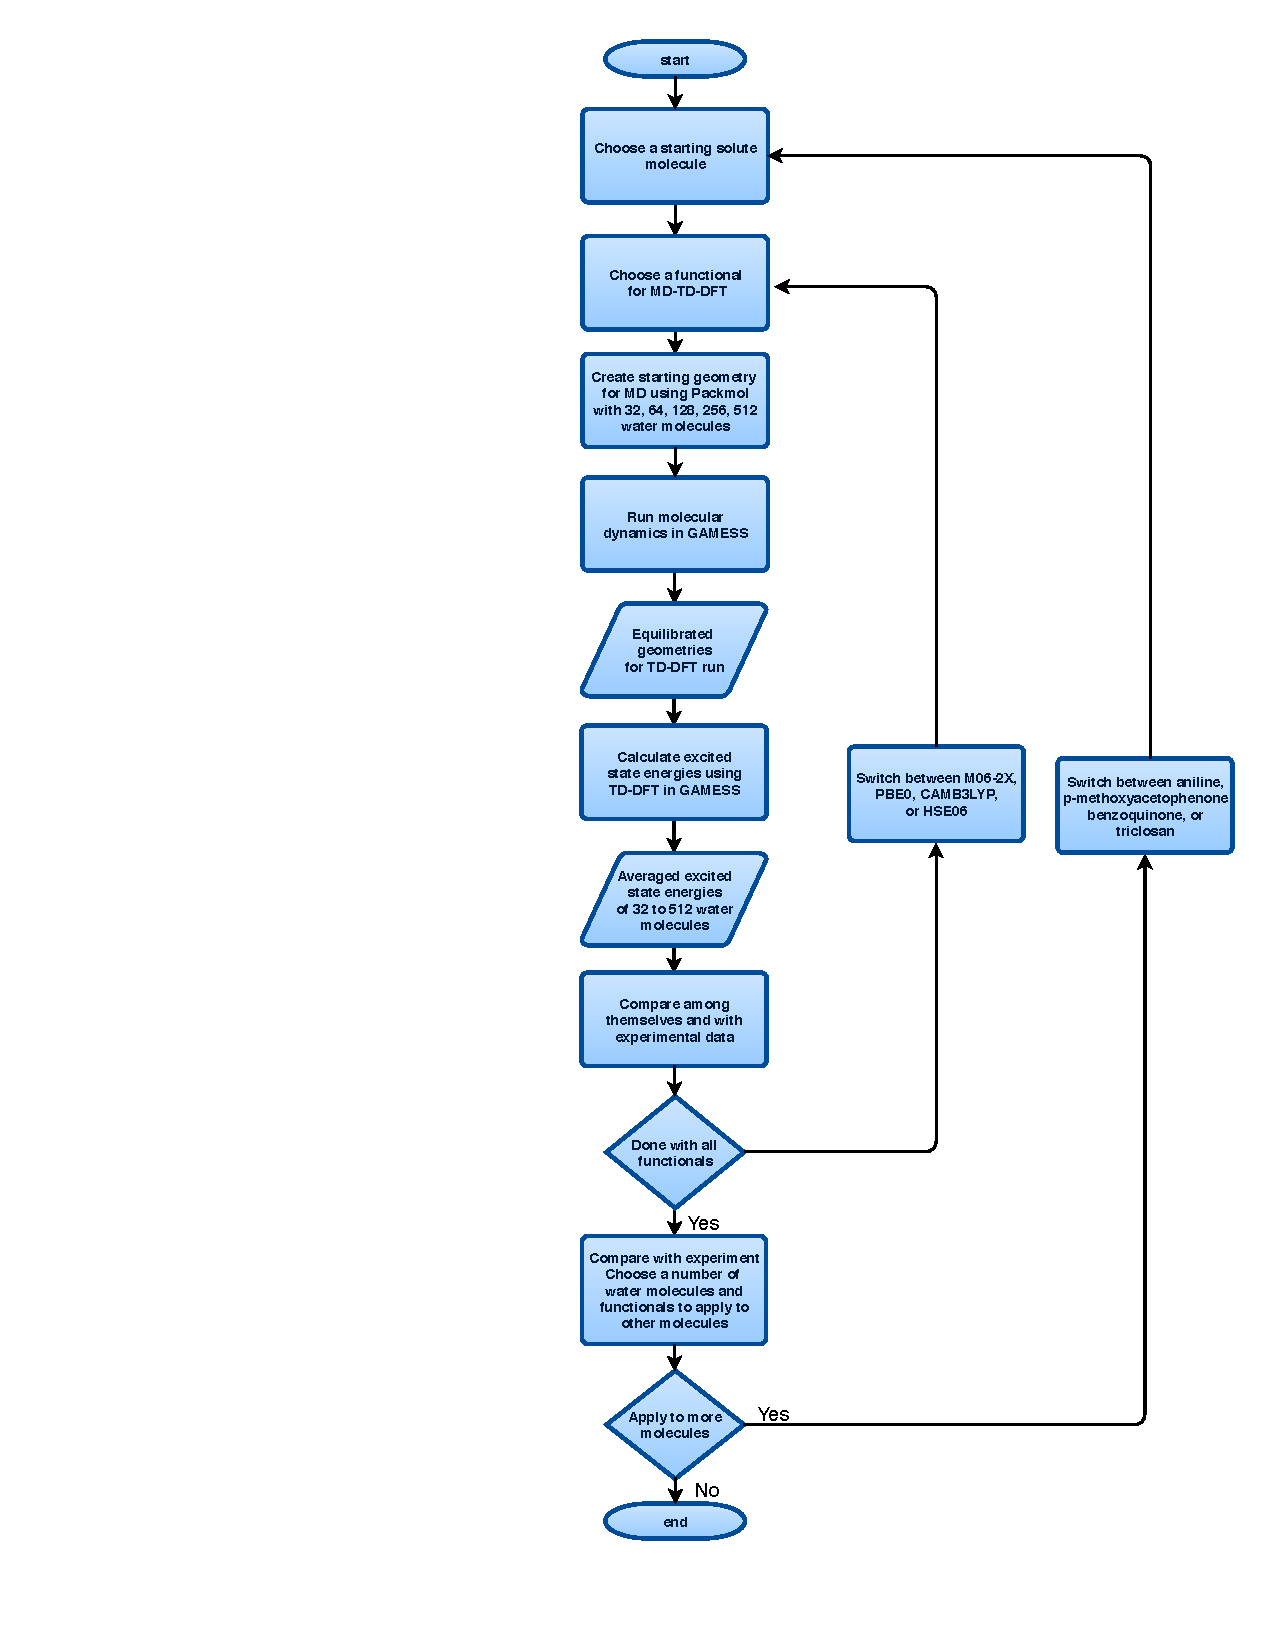
\includegraphics[width=0.9\textwidth]{flowchart.pdf}
	\caption{Flowchart of work in this project. Some of these processes are done using python scripts}
	\label{fig:flowchart}
\end{figure}

\subsection{Computational Models} 
Packmol was used to place water molecules around solute molecules to create starting geometry. GAMESS computational chemistry software was used in calculating MD and excited state energies. R was used to fit Gaussian under absorption spectrum, and integrate to find oscillator strength. In order to most accurately calculate the excited energies, the 6-311++G(2d,p) basis set is chosen to run single point energies on a set of equilibrated geometries. It has been decided to reduce the basis set in running MD, a smaller basis set 6-31+G(2d,p) will be used in order to cut computational cost. The decision comes as a suggestion from professor Soren Eustis after weeks of waiting for computational results when determining the number of water molecule in the model. Two best-performing DFT functionals out of all examined in previous study are explored: CAMB3LYP, M06-2X.\cite{Barnes2014} Either PBE0 or HSE06 will also be used to in future work.

The EFP model of water molecules is chosen to implement an explicit solvent model to calculate excited states energies. The appropriate number of water molecules to be included as EFP in the model has never been evaluated. Too many waters results expensive computational cost. Too few water will not fully model the solvent. A binary framework will be used to test how many water molecules are needed to fully solvate the solute environment: 32, 64,..512. Once excited state energies for each system are calculated, the results will be compared with experimental spectral data to find optimum number of waters before determining which functional should be chosen to achieve the most accurate computational model. 
\begin{figure}[!tbp]
	\centering
	\label{fig:startingGeometryAniline}
	\begin{subfigure}[b]{0.4\textwidth}
		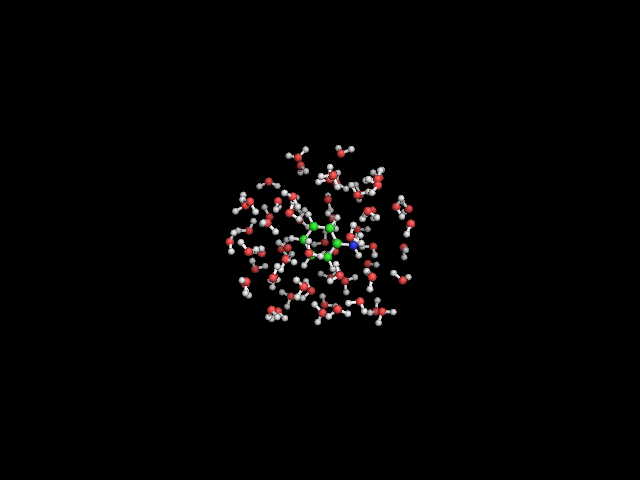
\includegraphics[width=1\textwidth]{startingGeometry/aniline64.png}
		\caption{}
		\label{fig:startingGeometryAnilinea)}
	\end{subfigure}
	\hfill
	\begin{subfigure}[b]{0.4\textwidth}
		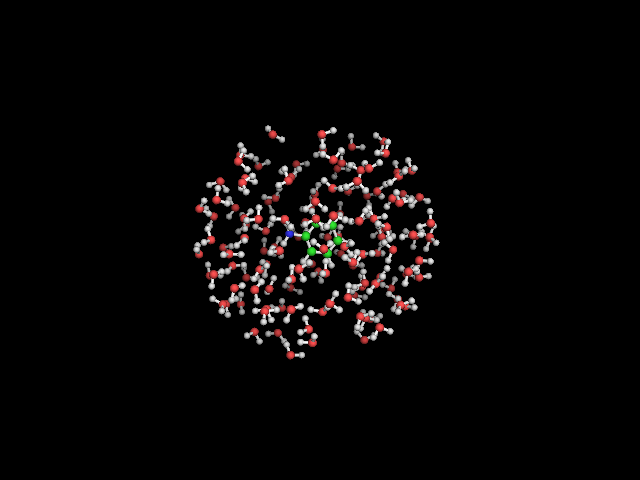
\includegraphics[width=1\textwidth]{startingGeometry/aniline128.png}
		\caption{}
		\label{fig:startingGeometryAnilineb)}
	\end{subfigure}
	\hfill
	\begin{subfigure}[b]{0.4\textwidth}
		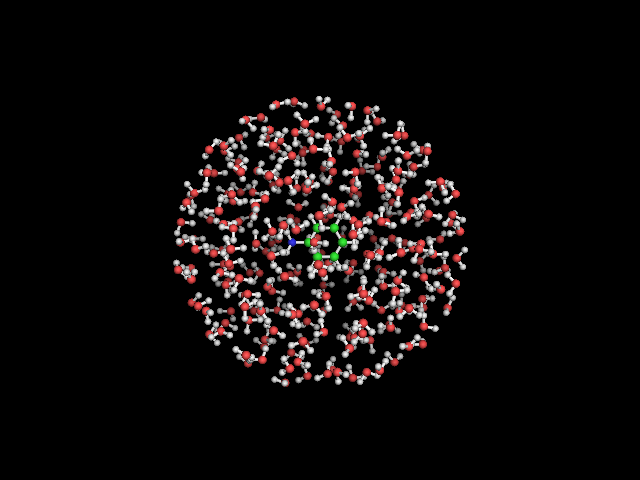
\includegraphics[width=1\textwidth]{startingGeometry/aniline256.png}
		\caption{}
		\label{fig:startingGeometryAnilinec)}
	\end{subfigure}
	\hfill
	\begin{subfigure}[b]{0.4\textwidth}
		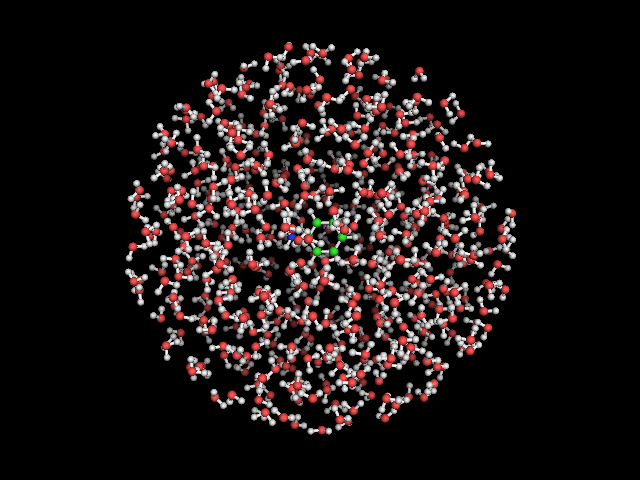
\includegraphics[width=1\textwidth]{startingGeometry/aniline512.png}
		\caption{}
		\label{fig:startingGeometryAnilined)}
	\end{subfigure}
	\caption{Binary approach to determining the right number of water in solvation sphere. Five numbers of water molecules between using 2\textsuperscript{n} with n=5-9 are used. a) 64 water molecules b) 128 water molecules c) 256 water molecules d) 512 water molecules}
\end{figure}
	
Aniline has been chosen as our initial test solute due to its hydrogen bonding capability, its small size, and extensive studies on aniline within Eustis lab. Successful model on aniline is likely to be applicable even to larger molecule with similar properties. After a model for aniline is decided, para-methoxyacetophenone and benzoquinone will be studied for their similarity in functionals to triclosan. Finally, the model will be applied to more known aquatic pollutants such as triclosan.

\section{Preliminary Results and Discussions}

Only aniline with 32 water with CAMB3LYP has excited state energy tabulated. Time was spent trying to fix bugs in GAMESS on Bowdoin HPC and ssbp problem. However, once everything is fixed, the process should run relatively smoothly for other functionals. Experimental absorption spectrum of aniline in water was collected by Alex and Holly over the summer of 2015. 

\section{Python Scripts}
Much of time was also spent on writing python scripts (see Appendix). In order to automatically generate input files and cultivate output data from output files, many python scripts are written from scratch. Since scripts are specific to each GAMESS run, there is a limited number of scripts available on the internet (virtually none for this project). Log files obtained from GAMESS contains both valuable experimental data and useless text strings. Python scripts play an important role in both data collection and smoothing up the process between each computational steps.  For example, even though WEBMO can generate sets of latest geometry in MD run, but retrieving geometry from each MD step requires one to manually open the log file and copy-paste the geometry into input files of the next step one by one. The python script postMDDataPull2.py is designed to pull thousands of geometries and generate GAMESS input files for TD-DFT energy calculation within seconds. Generating these python scripts will also allow unified program to be developed in order to automate the whole project without any manual input.

\subsection{Determining the equilibrium}
Determination of equilibrium was determined by eyeballing a plot of the solvent solute system's potential energy over time for a stable period as shown in the figure \ref{fig:MDEnergyAniline32d)}. The consistently low fluctuation indicates the start of equilibrium at 15000 fs. 1000 frames or 10000 fs of MD geometries were used to calculate the excitation energies in TD-DFT run.

\subsection{Determining the optimum solvent environment}
TD-DFT calculation for aniline with 32, 64, 128, 256, 512 surrounding water molecules were performed with CAMB3LYP basis set. Firstly, for 32 water molecules, the equilibrium were chosen to start from 15 ps and the stopping point of calculation was 25 ps; 1000 jobs for every 10 fs.  Geometry of the system though challenge the accuracy of 32-water model. Aniline molecule surrounded in 32 water molecules is unfortunately most stable not being fully solvated. Aniline can be seen outside of the water cluster at the time of equilibrium. This is in contrast to expected 32 water as the first solvation shell for aniline. \cite{Plugatyr2009} 

\begin{figure}[htb]
	\centering
	\label{fig:MDEnergyAniline32}
		 \begin{subfigure}[b]{0.4\textwidth}
		 	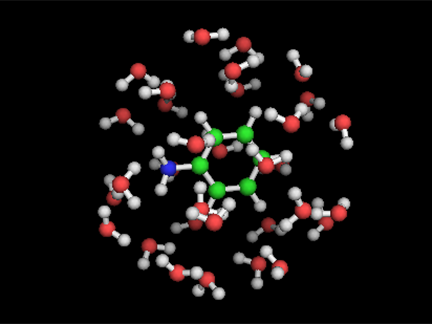
\includegraphics[width=1\textwidth]{CAMB3LYP/aniline32_0fs.png}
		 	\caption{}
		 	\label{fig:MDEnergyAniline32a)}
		 \end{subfigure}
		 \hfill
		 \begin{subfigure}[b]{0.4\textwidth}
		 	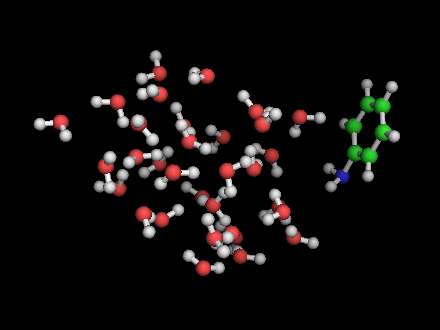
\includegraphics[width=1\textwidth]{CAMB3LYP/aniline32_15000fs.png}
		 	\caption{}
		 	\label{fig:MDEnergyAniline32b)}
		 \end{subfigure}
		 \hfill
		 \begin{subfigure}[b]{0.4\textwidth}
		 	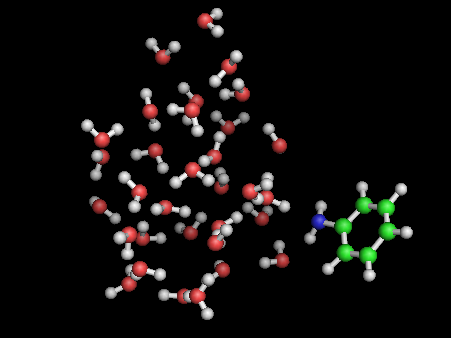
\includegraphics[width=1\textwidth]{CAMB3LYP/aniline32_25000fs.png}
		 	\caption{}
		 	\label{fig:MDEnergyAniline32c)}
		 \end{subfigure}
		 \hfill
		 \begin{subfigure}[b]{0.4\textwidth}
		 	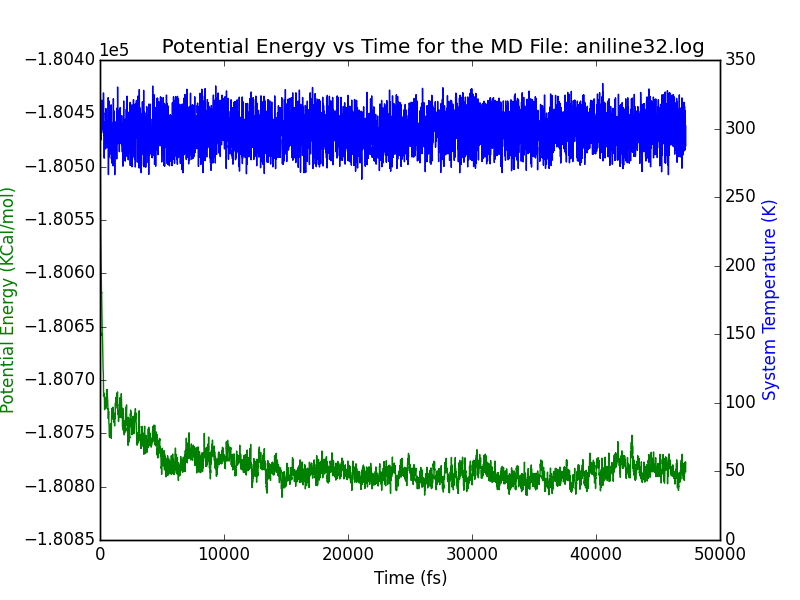
\includegraphics[width=1\textwidth]{CAMB3LYP/aniline32_EnergyPlot.png}
		 	\caption{}
		 	\label{fig:MDEnergyAniline32d)}
\end{subfigure}
\caption{Molecular Dynamics run of aniline in 32 explicit solvating water molecules. Notice that at equilibrium, aniline molecule comes outside of the water sphere. Albeit hydrogen bond being clearly established, lack of total submersion in water means 32-water does not fully solvate the aniline molecule and suggests that 64-water will give more accurate results. (a) starting geometry of MD run created by packmol. (b) geometry after 15000 fs. Notice the hydrogen bond between the amino group and water cluster. (c) geometry after 25000 fs. The amino group is pointing in the water sphere, as it continues to through out the whole MD run. (d) A plot of potential Energy of the system vs time. At 15000 fs, equilibrium starts as evident by decrease in energy fluctuation.}
\end{figure}

%for refing page number
%function grows near 0. Also, in the page \pageref{fig:mesh1}

\begin{table}[ht]
	\caption{Wavelength and Oscillator Strength from MD-TD-DFT calculation of aniline in 32 water molecules.}
	\label{table:aniline32TD-DFTTable}
	\centering
	\begin{tabular}{c c}
		Wavelength (nm) & Oscillator Strength\\ [1ex] % inserts table %heading
		\hline\hline
		\\[-0.5ex]
		173.00&0.165685\\
		180.20&0.364739 \\
		184.99&0.339029\\
		214.30&0.143915\\
		246.26&0.0383513\\ [1ex]
	\end{tabular}
\end{table}

The excited state energies and its oscillator strength from MD-TD-DFT calculation of aniline with 32 waters are tabulated in table \ref{table:aniline32TD-DFTTable}. Wavelength and oscillator strength from spectral data are tabulated in table \ref{table:anilineUVTable}. When compared with aniline's UVVIS spectra, as in figure \ref{fig:UVFromFityk}, there are several problems. Firstly, the calculated value at 246 nm does not accurately capture the peak at 230 nm and there is no calculated excitation energy at 280 nm, where the experimental peak is. The problem is probably due to aniline not being fully solvated. Nevertheless, two calculated wavelengths, 214.30 nm and 246.26 nm, identified with the experimental peak observed at 225 nm and 279 nm with comparable oscillator strength value.

Even though MD calculations for CAMB3LYP aniline64 through 512 have completed, no TD-DFT energies has been calculated as of now. 

\begin{table}[ht]
	\caption{Wavelength and Oscillator Strength calculated from experimental UV-VIS spectrum using Fityk, figure \ref{fig:UVFromFityk}. Notice the first peak does not have a maximum, this is due to the lower limit of the spectral data.}
	\label{table:anilineUVTable}
	\centering
	\begin{tabular}{c c}
		Wavelength (nm) & Oscillator Strength\\ [1ex] % inserts table %heading
		\hline\hline
		\\[-0.5ex]
		<200&>0.1298\\ 
		225&0.1699\\
		232&0.0570\\
		279&0.0274\\ 
	\end{tabular}
\end{table}

\subsection{Next steps}
Once energies and oscillator strengths of each solvent models are computed, data as a function of number of water can be evaluated. Aniline with 512 waters is the most time consuming system. If there is no significant improvement in comparison with 256 waters, this model will be discarded. 
In the future R code will be used instead of Fityk since Fityk requires manual insertion of underlying Gaussian plots. Elimination of this process will results in less manual input and more statistical approach to a statistical problem. Calulation using other functionals can be done relatively faster once the optimum number of water framework has been establish.

\clearpage
\appendix 
\label{appendix}
\section*{Appendix}
\renewcommand{\thesubsection}{\Alph{sub}}
	\subsection{Python Scripts}
		\subsubsection{Preparing MD Input Files}
			This script does two things. First (line 35-84), it calculates appropriate radius for solvent boundary potential. Some time and effort were spent on figuring out what the radius should be without emperically guess it. A simple model is proposed: At most solute will rotate around its outmost solute atom. This radius, in the code, is called solute radius. The other radius is solvent radius, its the distance between the outmost solvent atom to the solute's CG. These two radius plus an extra 2-3 Angstrom gives ssbp radius for MD input file. Second (line 87-155), the script parses xyz file's geometry data into MD input file. Slight format change is required for GAMESS input files, so this python code automate that change. The output file is MD file which can be run on GAMESS. Output of this script can be seen below in MD Input File section.
			\vfill
			\inputminted[linenos, breaklines, baselinestretch=1, fontsize=\small]{python}{../pythonScripts/prepareMD2.py}
		
		\subsubsection{MD Geometries extraction}
			One of the reasons, an MD run might fail is if solute molecule is pushed out of the water sphere. 3dExtract4.py allows geometries to be extracted into a xyz-movie file. xyz files, capable of containing more than one frame of geometries, allows one to follow MD through a combination of screenshot (each frame is 10 femtosecond - in the current MD input file - see MD Input File section). 
			\inputminted[linenos, breaklines, baselinestretch=1, fontsize=\small]{python}{../pythonScripts/3dExtract4.py}
			
		\subsubsection{Plot Potential Energy of MD run}
			plotEnergyMD6.py script is used to extract potential energy and temperature of each MD frame to determine the if the system has equilibrated. This and 3dExtract are very essential to the first stage of the project: they determine whether MD has failed or reached equilibrium based on the geometry and potential energy of the system. Many versions of this code has been developed and this is the most refined piece of code for its purpose. Future work can be done on plotting the plot on Matlab instead of obviously inferior python counterpart - matplotlib. 
			\inputminted[linenos, breaklines, baselinestretch=1, fontsize=\small]{python}{../pythonScripts/plotEnergyMD6.py} 	
		
		\subsubsection{Find The Most Equilibrated Period}
			There are currently no consensus as to when MD has reached the equilibrium. In the past, plotEnergyMD (previous script) was used to indicate whether the potential energy of the system(solute and solvent) has stabilized. Arbitrariness in deciding whether the equilibrium is reached falls in the hands of users. findEquilibrium.py is designed to solve this subjectivity. With a list of potential energies at different time from plotEnergyMD, linear fit can be done in a fix interval to evaluate the rise or fall in energy. Currently, the limit value is taken, still empirically, from 15000 to 25000 fs interval in CAMB3LYP aniline32.log. Further improvement can be done to find the bottom slope limit as a variable with molecule input.
			\inputminted[linenos, breaklines, baselinestretch=1, fontsize=\small]{python}{../pythonScripts/findEquilibrium.py} 
		
		\subsubsection{Prepare TD-DFT input}
			After equilibrium is determined, fincut2.py can be used to create TD-DFT input files from xyz-movie file. a Text file containing gmssub commands especially for Bowdoin hpc grid is created. The script was created by Nathan Ricke for this work, but many improvement has been made. The new script works faster and more efficient, even though it still has outdated syntax and methods.
			\inputminted[linenos, breaklines, baselinestretch=1, fontsize=\small]{python}{../pythonScripts/fincut2.py} 
		
		\subsubsection{Pull Excited State Energies from TD-DFT Log Files}
			postMDDataPull2.py pulls out excited state energies and dipole moments. Energy output is in the format of time, S1, S2... Dipole output is in the format of time, X1, Y1, Z1, X2...
			\inputminted[linenos, breaklines, baselinestretch=1, fontsize=\small]{python}{../pythonScripts/postMDDataPull2.py} 
		
	\subsection{GAMESS inputs}
		\subsubsection{MD Input File}
			 MD run is core to modeling explicit solvent. The MD run is simulated every femtosecond but only record every 10 femtoseconds. The bath temperature is 25 $\pm$ 25 degree Celsius. Solvent boundary potential is also actiavetd using default Sforce value, but with estimate ssbp radius. \#\#\#\#\#\#\#\#\#n\#\#\#\#\#\#\#\#\# are for restarting MD in case the calculation abruptly ends (see next section). In this version, dispersion correction is not turned on. Basis set = 6-31+G(2d,p)
			 \inputminted[linenos, breaklines, baselinestretch=1, fontsize=\small]{Perl}{../GAMESSinpSample/MD_aniline32.inp}
			 
		\subsubsection{MD Restart}
		\#\#\#\#\#\#\#\#\#n\#\#\#\#\#\#\#\#\# are for restarting MD. For example, if MD stops from errors at t= 39000 fs, a restart geometry and \$MD should be obtained from t= 38960 in the run's trj file. \#\#\#\#\#\#\#\#\#1\#\#\#\#\#\#\#\#\# from trj goes to \#\#\#\#\#\#\#\#\#1\#\#\#\#\#\#\#\#\# in MD input file and so on with 2 and 3.
		\inputminted[linenos, breaklines, baselinestretch=1, fontsize=\small]{Perl}{../GAMESSinpSample/MD_aniline32.trj}
		
		\subsubsection{TD-DFT Input File}
			Excited state energies are calculated using TD-DFT. Direct SCF calculation is turned on. Basis set = 6-311++G(2d,p)
			\inputminted[linenos, breaklines, baselinestretch=1, fontsize=\small]{Perl}{../GAMESSinpSample/TDDFT_aniline32_15010.inp}


\acknowledgement

Sed aliquam euismod nunc nec consectetur. Fusce eget dui id tortor tristique luctus. Pellentesque elit eros, molestie et molestie vitae, laoreet in risus. Nullam ligula lectus, pulvinar eget sagittis sed, cursus ac magna. \ldots


\suppinfo

Ut volutpat, felis sit amet malesuada blandit, arcu sapien feugiat libero, vel interdum ipsum dolor et dolor. Fusce tortor sapien, pharetra sit amet posuere ac, viverra mollis est. Maecenas auctor ultrices quam a pharetra. Aenean ornare dictum libero vitae gravida. Mauris auctor sapien at purus accumsan lacinia.

\bibliography{citation.bib}

\end{document}
